\chapter{Blocks}\label{chapter:blocks}

\section{The Network Delay}

In the last chapter, we created a monetary system in which participants can issue transactions
and transfer money between one another while maintaining scarcity. We ensured participants can
only spend their own money by using an unforgeable signature scheme to authenticate transactions
that everyone verified. By gossiping transactions on the network, every participant assembled
them, upon verification, into a transaction graph, and reading the UTXO set of that transaction
graph enabled participants to determine \emph{who owns what}.
Furthermore, we made that transaction graph append-only. Our intuition is that, since every
transaction is gossiped, everyone will eventually arrive at the same transaction graph,
and the population will reach consensus on the UTXO set, even if some transactions take
a moment to arrive to distant parts of the network. Note that, it doesn't matter to us if
different honest parties observe transactions arriving on the network in different order,
as long as all the parties compute the same UTXO set. This is the only thing that's important
to determine \emph{who owns what}. If two honest nodes accept the same set of transactions,
even if they have processed them in different order, they will arrive at the same transaction
graph and the UTXO set computed by them will be the same.

Of course, if a transaction is delayed while in transit on the network \emph{for ever}, some nodes
will not receive it and they will not be in consensus with the rest of the network, but this
contradicts our non-eclipsing assumption that we introduced in
Chapter~\ref{chapter.untrusty-world}. To make our intuition more precise, let us quantify how
long it takes for a message to reach the whole network when it is broadcast by any party.
We call this the \emph{network delay parameter}.

% TODO: Explain \Delta with reference to the network topology / network diameter
\glsxtrnewsymbol[description={network delay}]{delay}{$\Delta$}\glsadd{delay}
\begin{definition}[Network Delay]\index{Network Delay}
  The \emph{network delay parameter} $\Delta$ measures the maximum time it takes
  for a message to travel from one honest party to every other honest party on the
  network.
\end{definition}

Because honest parties gossip adversarial messages, this network delay ensures that
even adversarial messages make it across the network within $\Delta$ time. That is,
if an honest party receives an adversarial message at some point in time, then every
honest party will see the same adversarial message within time $\Delta$.

Now we can express our intuition that nodes reach consensus more precisely:
While some transactions may be delayed up to $\Delta$ time,
if no transactions are broadcast for a time of $\Delta$, everyone's transaction
graph will converge to be the same, and the UTXO set will be shared among along
all honest parties. Unfortunately, this intuition is misguided, and things are not
that simple. Things break down when double spend transactions are introduced
by the adversary.

\section{The Double Spend}\index{Double Spend}

Let's try to understand the double spending problem a little more carefully. Eve
receives $1$ unit of money from Alice through a transaction $\tx_1$ as illustrated in
Figure~\ref{fig.double-spend}. The transaction $\tx_1$ was created honestly by Alice
and has one input of $1$ unit coming from Alice, and one output of $1$ unit paying
Eve's public key. Eve now creates two transactions: The first transaction, $\tx_2$
consumes the single output of $\tx_1$ and pays $1$ unit back to Alice. The second transaction,
$\tx_2'$ also consumes the single output of $\tx_1$ and pays $1$ unit, this time to Eve.

Suppose that two other parties, Charlie and Dave, have already seen $\tx_1$ on the network,
but have not yet received either of $\tx_2$ or $\tx_2'$. If Charlie receives $\tx_2$, he
will accept this transaction as valid. The transaction's input contains an outpoint that
points to an element of the UTXO set in his view, since the output of $\tx_1$ has not been
previously spent. Furthermore, the transaction contains a valid signature by Eve created
with the correct secret key, and it satisfies the Conservation Law. Upon accepting $\tx_2$,
Charlie updates his UTXO set, removing the output of $\tx_1$ and adding the output of
$\tx_2$ to it. If Charlie now receives $\tx_2'$, he will reject this transaction, as
it is spending from an output that is not in the UTXO set in his view.

On the contrary, Dave receives $\tx_2'$ first, and $\tx_2$ after. When Dave receives $\tx_2'$,
he considers this a valid transaction, because it is spending from the UTXO set in his view.
Dave, contrary to Charlie, believes that the output of $\tx_1$ is still in the UTXO set.
Dave then updates his UTXO set, removing the output of $\tx_1$ and adding the output
of $\tx_2'$ to it.

At this point Charlie's and Dave's view are in disagreement. This is a problem. If Alice has
also received $\tx_2$ prior to $\tx_2'$, she will justifiably believe that Eve paid her.
While Charlie will accept Alice's money, because it is in his UTXO set, Dave will not accept
Alice's money. We have arrived at a situation where Alice's money is not acceptable to everyone.
We have lost consensus on \emph{who owns what}.

\begin{figure}[h]
    \centering
    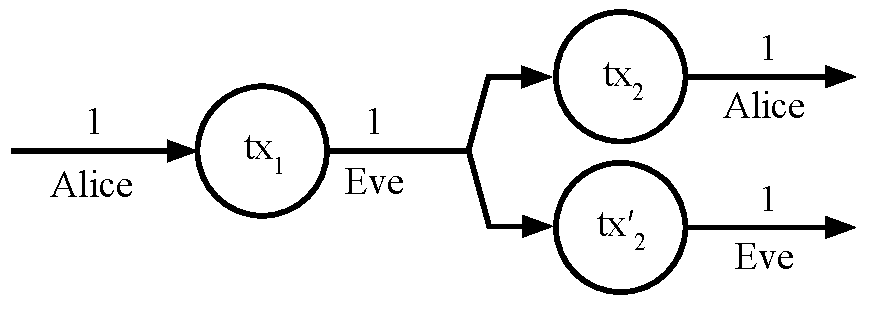
\includegraphics[width=0.6 \columnwidth,keepaspectratio]{figures/double-spend.pdf}
    \caption{A double spend transaction. Alice paid Eve $1$ unit through $\tx_1$, but Eve spent it in both $\tx_2$ and in $\tx_2'$,
             which have different recipients.}
    \label{fig.double-spend}
\end{figure}

\section{Simple Ideas Don't Work}\label{sec:simple-ideas}

Let us consider three simple ideas to resolve the double spending problem that first come to mind.
Sadly, these ideas won't work.

\begin{figure}[h]
    \centering
    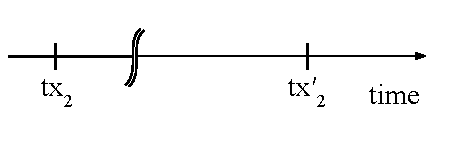
\includegraphics[width=0.4 \columnwidth,keepaspectratio]{figures/simple-idea-1.pdf}
    \caption{The first idea is unviable because it allows the
    adversary to retroactively invalidate an earlier transaction much later. Here, $\tx_2'$
    is initially withheld, but broadcast much later, causing an invalidation to the earlier
    $\tx_2$ transaction.}
    \label{fig.simple-idea-1}
\end{figure}

\noindent
\textbf{Idea 1: Reject double spends altogether.} Honest parties never double spend. Since the adversary is the only one
creating double spends, why do we need to provide any assurances? We can opt to simply invalidate that
money. We add the following rule to our protocol:

\begin{quote}
If you see a transaction that is a double-spend,
then consider \emph{all} of the transaction outputs that pertain to the double spend transactions invalid.
\end{quote}

This approach is problematic. The reason is that the adversary can retroactively take back
a payment: She initially broadcasts $\tx_2$ to the network paying Alice, but keeps $\tx_2'$ withheld,
as illustrated in the timeline of Figure~\ref{fig.simple-idea-1}.
Alice, like everyone else, observes $\tx_2$ on the network, but not $\tx_2'$. She thinks this is
a normal transaction and accepts the payment. In exchange for this payment, Alice provides a service
to Eve: she serves her coffee. At a later time, Eve has enjoyed the coffee and has departed from Alice's
establishment. At this point, Eve broadcasts $\tx_2'$, a double spend of $\tx_2$. Suddenly, everyone
on the network considers both $\tx_2$ and $\tx_2'$ invalid. Alice's money is gone. Therefore, we cannot
adopt this construction.

\begin{figure}[h]
    \centering
    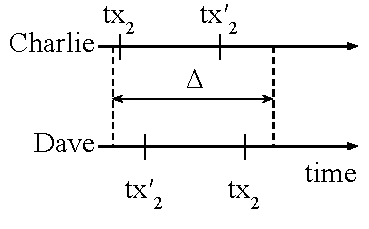
\includegraphics[width=0.325 \columnwidth,keepaspectratio]{figures/simple-idea-2.pdf}
    \caption{The second idea is unviable because parties
    have views in disagreement about transaction order. Here, Charlie believes $\tx_2$
    precedes $\tx_2'$, whereas Dave believes $\tx_2'$ precedes $\tx_2$.}
    \label{fig.simple-idea-2}
\end{figure}

\noindent
\textbf{Idea 2: Accept the first transaction seen.} As we saw, two different honest parties can disagree on
the order in which two transactions arrived on the network. The situation is illustrated in
Figure~\ref{fig.simple-idea-2}. Therefore, the following simple construction does not work:

\begin{quote}
  Among double spending transactions, accept the first, and reject every subsequent transaction.
\end{quote}

However, we now note that these two transactions must be broadcast
to honest parties in close succession, and in particular within time $\Delta$. If the adversary
were to reveal $\tx_2$ to Charlie first, but then wait for more than $\Delta$ time until she revealed
$\tx_2'$ to Dave, then Charlie would have gossiped $\tx_2$ and Dave would have receive it within $\Delta$
and prior to seeing $\tx_2'$. In that case, Charlie and Dave would be in agreement.
In order for the adversary to cause disagreement, she must broadcast the two double spending
transactions to two different honest parties within time $\Delta$ of each other. Yet, this is
simple for an adversary to do, so we cannot adopt this construction either.

\begin{figure}[h]
    \centering
    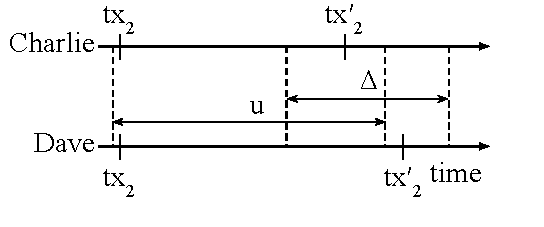
\includegraphics[width=0.45 \columnwidth,keepaspectratio]{figures/simple-idea-3.pdf}
    \caption{The third idea is unviable because parties
    disagree about whether $\tx_2$ and $\tx_2'$ have arrived within time $u$,
    and follow different policies. Here, Charlie rejects both transactions, whereas
    Dave accepts $\tx_2$ and rejects $\tx_2'$.}
    \label{fig.simple-idea-3}
\end{figure}

\noindent
\textbf{Idea 3: Reject double spends within $u$.} Why don't we combine ideas 1 and 2? We saw that
Idea 1 is problematic because it allows the adversary to retroactively take back a transaction after
a long time into the future. We also saw that Idea 2 is problematic because it allows an adversary to
cause disagreement when two transactions are broadcast in close succession. This creates a natural
new construction idea:

\begin{quote}
Upon seeing a transaction, wait for some time $u \geq \Delta$. If a double spend
appears within the window $u$, reject all double spending transactions. However, if $u$ has passed and we have
not seen any double spends, accept the single transaction that we have seen. If a double spend appears in
the future, just reject that one.
\end{quote}

At first sight, this third idea seems to work: After time $u$ has passed, either the money is accepted or not.
The adversary cannot walk away as she did against Idea 1. If the adversary broadcasts two conflicting
transactions within $\Delta$ time, as she did against Idea 2, they will both be rejected. It won't matter
that different parties saw them in different order.

Sadly, upon closer inspection, this idea does not work,
either. The strategy of the adversary is now to cause disagreement between Charlie and Dave with
regards to \emph{whether or not} the two transactions appeared within time $u$. The problematic situation
is illustrated in Figure~\ref{fig.simple-idea-3}. The adversary initially broadcasts $\tx_2$
to both Charlie and Dave. Both Charlie's and Dave's clocks start ticking to measure the time $u$.
Right before time $u$ hits, the adversary broadcasts $\tx_2'$ to Charlie. Now, Charlie has seen
a double spend within time $u$, and so he rejects both $\tx_2$ and $\tx_2'$. He also rebroadcasts
$\tx_2'$ to Dave, but this message will require time $\Delta$ to reach Dave. In the meantime,
time $u$ has passed, and Dave accepts $\tx_2$. When $\tx_2'$ arrives on Dave's end, Dave has
already accepted $\tx_2$ and now rejects $\tx_2'$. Now Charlie and Dave are in disagreement:
Dave thinks $\tx_2$ is valid, whereas Charlie thinks $\tx_2$ is invalid.

Try to think of more simple ideas to resolve this ordering issue. You'll see that
none of them will work. For example, placing a timestamp within a transaction to ensure
that every honest party simultaneously applies a transaction doesn't work, either (why?).
Neither does the policy of accepting the transaction with the smallest $\txid$ among
double spends (why?).
We'll need to invent heavier artillery to attack this problem. Over the next few
sections, we'll gradually derive the concepts of a \emph{block} and a \emph{chain}.
While we do this, we will find issues with our scheme and keep augmenting it until
we arrive at a fully working safe and live protocol.

\section{Ledgers}

Even though honest parties receive transactions in a different order on the network,
we would like to have them coordinate with one another to report them in the same
order. Each honest party will report a \emph{ledger}, an ordered sequence of transactions.
This ledger will not necessarily contain the transactions in the order they were
received from the network. It may also not immediately report some transaction as
soon as it is received from the network, but, akin to Idea 3 of Section~\ref{sec:simple-ideas},
it may need to delay reporting it on its ledger for a bit.
By reading that ledger reported by an honest party one transaction at a time from left to right,
we can reconstruct the transaction graph and arrive at the UTXO set. If the honest parties
agree on their reported ledgers, they will agree on the UTXO set. We'll therefore concern
ourselves with the question of whether we can achieve consensus among the ledgers reported
by honest parties.

We will soon figure out what each honest party should do internally in order to produce
a ledger that is consistent with every other honest party, but before we get to \emph{how}
to do that, let us first more clearly articulate what exactly it is that we want to achieve.

We wish to build an honest party construction $\Pi$ which we call the \emph{full node}\index{Full node}.
This will be a piece of code which will be identically executed by all honest parties.
It will implement peer discovery, the
gossiping network communication to exchange messages on the network, and so on. In
addition, we'll make $\Pi$ expose two functionalities: A
\emph{write} functionality, and a \emph{read} functionality. The \emph{write} functionality
accepts a brand new transaction. This transaction is
broadcast and gossiped to every other party on the network by the full node.
The \emph{read} functionality returns a ledger of transactions.
These functionalities are used by the \emph{wallet}. Together, the full node and
the wallet constitute the software that is running on the human user's machine.
The human user only interacts with the wallet, while the full node sits on the backend.

The wallet is a piece of software that is capable of creating and signing
new transactions to make payments as instructed by the user. The wallet also shows
whether a payment was received, and displays the balance of the user. These functionalities
are made possible by having access to the \emph{write} and \emph{read} functionalities
exposed by the full node. The \emph{write} functionality is what the wallet uses to
broadcast a new transaction into the network, whereas the \emph{read} functionality
allows the wallet to obtain a ledger that it can then use to obtain the UTXO set
in order to display whether a payment has been completed and to calculate the user
balances. This architecture is illustrated in Figure~\ref{fig.wallet-fullnode-architecture}.

\begin{figure}[h]
    \centering
    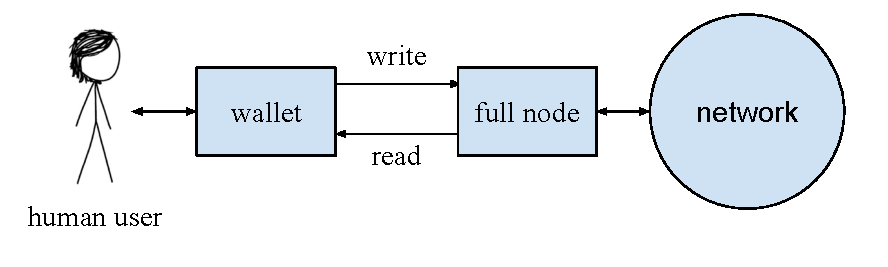
\includegraphics[width=0.65 \columnwidth,keepaspectratio]{figures/wallet-fullnode-architecture.pdf}
    \caption{The human user interacts with the wallet. The wallet interacts with the full node
    by invoking its \emph{write} and \emph{read} functionalities. The full node interacts with the network.}
    \label{fig.wallet-fullnode-architecture}
\end{figure}

We'll have more to say about the wallet portion in the next chapters. For now,
let us focus on how to build the full node.
Our goal will be to have all the honest full nodes agree on the ledgers they are reporting
when their \emph{read} functionality is invoked. That way, everyone will arrive at the same
UTXO set and agree \emph{who owns what}.

\begin{definition}[Ledger]
    A \emph{ledger} of an honest party $P$ reported at time $r$, denoted $L^P_r$ is
    a finite \emph{sequence of transactions} returned when the honest party $P$ invokes
    the \emph{read} functionality of its honest protocol $\Pi$.
\end{definition}

We take note here that ledgers are dependent on both $P$ and $r$. It is nonsensical to
speak about ``the ledger'' without specifying \emph{who} and \emph{when}. While these
parameters may sometimes be implicit, it is imperative that we understand what we are
talking about. Ignoring the \emph{who} and the \emph{when} of the ledger, and speaking
about ``the ledger'' as if it is a global view, is a common cause for confusion and
misconception. As we saw in the previous section, the ledgers of different honest
parties may be in disagreement, and there might not even be a well-defined global
ledger.

We want the ledgers reported by honest parties to have two \emph{virtues}. We give
an intuitive definition of these virtues now, but we will return to define them
more formally in Chapter~\ref{chapter:earnest2}.

\begin{definition}[Safety (informal)]
    For any two honest parties, their reported ledgers at any point in time
    are be equal.
\end{definition}

\begin{definition}[Liveness (informal)]
    If an honest party \emph{writes} a transaction into its ledger, then this
    transaction appears in the ledgers of all honest parties ``soon''.
\end{definition}

Let us think what these virtues are saying. If a ledger has \emph{safety},
then \emph{bad things don't happen}. We do not run into double-spend situations,
or into disagreements about \emph{who owns what}. If a ledger has \emph{liveness},
then \emph{good things happen}. When an honest party attempts to issue a transaction,
this transaction actually does take place.

It is easy to build a protocol that has \emph{safety} or \emph{liveness}, but not
both together.

\noindent
\textbf{Safe but not live.} A safe but not live protocol acts as follows.
Whenever the \emph{read} functionality is invoked, it returns the empty sequence of
transactions as the ledger. Whenever the \emph{write} functionality is invoked, it
ignores the transaction being written. It never reads or writes anything from the
network. Because the \emph{read} functionality always returns the same thing,
safety is trivially satisfied. Liveness, however, is not satisfied. When an honest
party attempts to make a transaction, it is never reported in the ledgers of other
honest parties.

\noindent
\textbf{Live but not safe.} A live but not safe protocol acts as follows.
Each honest party begins with an empty initial ledger. Whenever the \emph{write}
functionality is invoked with a transaction, this transaction is appended to the
local ledger and broadcast to the network. When a new transaction is received from the
network, it is gossiped to the rest of the network and appended to the local ledger.
The \emph{read} functionality returns the local ledger. This protocol is live
because every honest transaction makes it to the ledger of every honest party.
However, it is not safe, because transactions are reported on the ledgers in the
order they are received from the network, and this order may be different for
different parties.

Our design goal for the rest of this book will be to build protocols that
are \emph{both} safe and live simultaneously.

\section{Rare Events}
We previously determined that the root cause of double spending transactions being problematic
is because the adversary can issue them in short succession, and in particular within time
$\Delta$. It would be useful to enforce that the adversary issues transactions at a slower
rate. We'd like to limit the rate at which the adversary can issue transactions at
once every $\Delta$, with \emph{periods of silence} in between. If transactions are
spaced apart by $\Delta$ time, then no harm can come from double spends. We can simply
adopt the strategy of accepting the first among multiple double spending transactions,
and ignoring subsequent double spends.

To force the adversary to issue transactions $\Delta$ apart, we'd like to require her
to obtain a \emph{ticket} before she can issue a transaction, and each of these tickets
should be obtained every $\Delta$ time. Then, when she issues a transaction, the adversary
will be required to associate the transaction with the ticket, and that will cause the
ticket to be expended. The same ticket cannot be used for multiple transactions. Of course,
our protocol does not know who is adversarial and who is honest and must treat everyone
equally, so the ticket system applies to honest and adversarial parties alike.

If our tickets are issued more often than $\Delta$ apart, this will not be a good protocol,
as double spends will still be possible, harming safety. On the contrary, if our tickets
are issued much longer than $\Delta$ apart, the honest parties will take a long time to issue
transactions, and liveness will deteriorate. The choice of how often to allow tickets to be
issued highlights a theme that we will keep returning to throughout this book: A trade-off
between safety and liveness. This trade-off is illustrated in Figure~\ref{fig.time-tickets}.

\begin{figure}[h]
    \centering
    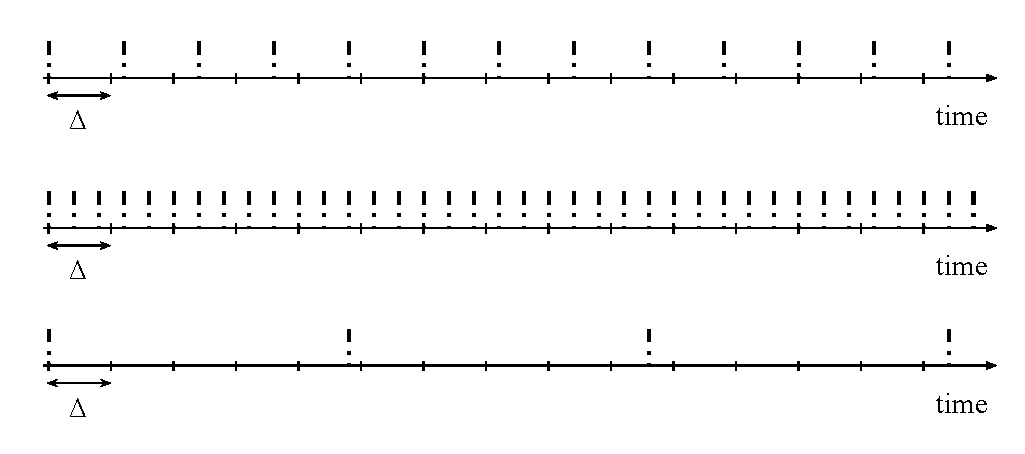
\includegraphics[width=0.8 \columnwidth,keepaspectratio]{figures/time-tickets.pdf}
    \caption{Positioning tickets in time. Tickets spread apart by slightly more than $\Delta$ (top)
             achieve good safety and liveness. Tickets spread apart less than $\Delta$ (middle)
             can cause safety violations. Tickets spread apart much more than $\Delta$ (bottom)
             cause liveness to deteriorate.}
    \label{fig.time-tickets}
\end{figure}

But how can we create such a ticketing system? How can we get them to behave this way in a permissionless
world, where there is no authority to issue these tickets and ensure they are spread $\Delta$
apart?

\section{Proof-of-Work}

There is a natural candidate for creating rare events like the tickets we need in a permissionless
world. When we introduced hashes in Chapter~\ref{chapter:primitives}, we gave a brute-force algorithm
(Algorithm~\ref{alg.hash-preimage})
that breaks the preimage property of a hash, but takes exponential time. However, we can tweak
the problem of finding a preimage so that it is not an \emph{exact} preimage, but a ``close enough''
solution. This will allow us to create a problem that is \emph{moderately hard}; it is not \emph{hard}
in the computational sense, but we can tweak how long it takes to solve it. We are interested in
``close enough'' hash preimages of the image $h = 0$; that is, we want an input $B$ to the hash function
$H$, so that $H(B)$ is a small enough number. \emph{How close} is defined by the value $T$, the
\glsxtrnewsymbol[description={target}]{target}{$T$}\glsadd{target}\emph{target}\index{Target}.
We write this requirement in the form of an
inequality:

\[
    H(B) \leq T
\]

This inequality is known as the \emph{proof-of-work inequality}\index{Proof-of-Work}. Finding
a $B$ that satisfies this equality is known as \emph{performing work}.
Remember
that the output of the hash function $H(B)$ is a $\kappa$-bit binary number. We are comparing
this number against the value $T$, another number. The inequality is satisfied if $H(B)$, treated
numerically, is not larger than the number $T$.

The challenge is to find the unknown value $B$ so that the inequality is satisfied. Of course,
there will be multiple $B$ values that satisfy this inequality. Upon solving this inequality,
one obtains a ticket to issue a transaction. While solving the inequality is moderately hard,
and requires many trial-and-error invocations of the hash function, verifying that the particular
$B$ satisfies the equation is very easy: It requires just one hash invocation.

\import{./}{algorithms/alg.proof-of-work}

To find a ticket, one can execute a strategy similar to the exhaustive search for finding a
preimage. We start at a random $B = \ctr$ and keep looking for a $\ctr$ that satisfies the
proof-of-work inequality by incrementing $\ctr$ and checking whether the equation is satisfied.
This is illustrated in Algorithm~\ref{alg.proof-of-work} and is known
as \emph{mining}\index{Mining}. The value $\ctr$ is known as the
\emph{nonce}\index{Nonce}\glsxtrnewsymbol[description={nonce}]{nonce}{$\ctr$}\glsadd{nonce},
and has no significance beyond ensuring that the proof-of-work inequality is satisfied.
Once a party finds a ticket $B$, this ticket can be gossiped
to the network and relayed by others. Any party can check that the ticket has a valid proof-of-work,
without performing the exhaustive search again. Intermediary nodes on the gossip network cannot
modify the contents of a ticket in transit, as this will invalidate the proof-of-work, and they
would have to mine a new ticket.

The larger we make the target $T$, the easier it is to solve the inequality. The smaller we make
the target $T$, the more difficult it becomes. That's why we call the value $\frac{1}{T}$ the
\emph{difficulty}\index{Difficulty}: The larger the difficulty, the more difficult it is to
find a solution to the inequality. By increasing $T$, we space tickets closer together.
By decreasing $T$, we space tickets further apart from each other. At the extremes,
setting $T = 0$ makes the proof-of-work problem equivalent to finding the hash preimage of
$0$, which needs exponential time. On the other end of the spectrum, setting $T = 2^\kappa$
makes the proof-of-work problem trivial, because every hash satisfies the inequality
$H(B) \leq 2^\kappa$.

\section{The Block}

We have introduced a moderately hard problem that forces the adversary to spread out her
tickets in time by more than $\Delta$. But how do we associate tickets with transactions?
We cannot just require the adversary to send a ticket together with a transaction.
The adversary may reuse a ticket multiple times, or may use a ticket together with one transaction
when communicating with one party and the same ticket with another transaction when
communicating with another party. We need to somehow tie the ticket together with a
transaction so that a ticket is only usable for a particular transaction.
To do this, we set $B = \tx \conc \ctr$ and require the ticket to satisfy $H(B) \leq T$,
as before, where $\tx$ is the transaction we want the ticket to be tied to.
The notation $\conc$ denotes the concatenation of two strings (separating them appropriately
so that they don't accidentally mix with each other by using an appropriate encoding such
as JSON).
Now, upon receiving a transaction/ticket pair, we can check that the ticket corresponds
to the particular transaction. Furthermore, if the adversary attempts to replace the
transaction within $B$ with a different one, then this will cause $H(B)$ to change.
The value $H(B)$ is \emph{committing} to a particular transaction; changing the transaction
changes the value $H(B)$ in a way that cannot be predicted. If she changes the transaction,
this will invalidate the proof-of-work and the adversary will have to perform yet another
exhaustive search to find a new ticket.

We've solved one problem, but have introduced another: If we require one ticket per transaction
for the adversary, then we must do the same for the honest parties. This means that at most one
transaction can be executed every $\Delta$. If the honest party wants to issue multiple transactions,
this will take a long time, and liveness will deteriorate. In order to solve this, we will \emph{bundle}
transactions together into a sequence $\overline{x} = (\tx_1, \tx_2, \ldots, \tx_n)$, and place
this within the ticket, setting $B = \overline{x} \conc \ctr$.
Instead of each ticket being associated with \emph{one} transaction, each ticket
Such a ticket is known as a \emph{block}\index{Block}.
Now each honest party can issue as many transactions
as he wants in one go, as long as he is able to mine one block.
From now on, we will no longer speak of tickets, but will speak of blocks,
even if a block contains just one transaction.

A natural question now arises: If we've bundled multiple transations together into one block,
hasn't the double spending problem resurfaced? The answer is \emph{no}, because, in order to
verify a block, all the transactions must be sent together in the bundle. As part of our block
validation rule, we will require that there are no conflicting transactions within the payload
$\overline{x}$ of a block. If $\overline{x}$ contains two mutually double spending transactions,
the whole block will be rejected. Blocks are either accepted or rejected as a whole. We will not
partially accept transactions within a block.

Double spending transactions can still appear in different blocks, but the moderate difficulty
of the proof-of-work puzzle ensures that blocks are produced sufficiently far apart. Like
transactions, blocks are gossiped over the network. If two blocks are transmitted at least
$\Delta$ time apart, then the first will arrive at the doorstep of every honest party before
the second. The second block, containing a transaction that double spends a transaction in the
first block, can then be rejected by all honest parties. Again, here, the whole block will be
rejected, not just the particular pathological transaction.

\section{The Mempool}

Even though we allow each mining party to include many transactions into their own blocks,
honest parties are still encumbered with the responsibility to mine a block before they can
get their transactions accepted by others. This wait time may still be long and this scheme
is not very good for liveness. Worse yet, some honest parties may have large computational
power, while other honest parties may have smaller computational power, and so the block
generation time for each honest party might be vastly different. It would be nice if we didn't
tie the liveness of each honest party to that particular party's computational power, but
instead allowed the honest parties to work together to confirm each others' transactions.

Towards that purpose, we design the system as follows: A transaction can still be issued
independently of a block and broadcast to the network. The transaction is gossiped until
it reaches everyone on the network as usual. However, the transaction is placed into a
temporary waiting area called the \emph{mempool}~\index{Mempool}, ensuring double spends are
resolved one way or another (any of the simple ideas we discussed previously can be used as
strategies to resolve double spends).
Each honest party maintains their own mempool $\overline{x}$ of transactions that are still in limbo.
Because the double spending problem has not yet been solved by finding a block, different
honest parties may disagree about what their mempool looks like.
However, each mempool is independently locally consistent.

\begin{definition}[Mempool]
    The \emph{mempool} $\overline{x}$ of an honest party $P$ at time $r$ is the sequence of transactions
    that have been received and validated, but have not yet been included in a block.
\end{definition}

Upon receiving a transaction from the network, an honest party performs the usual transaction
validation checks on it before adding the transaction to its own mempool, so the mempool
does not contain double spends. Of course, the mempool of one honest party may contain a
transaction which conflicts another transaction in the mempool of another honest party.
As honestly generated transactions can always be appended to the transaction graph,
the mempool of every honest party will contain every honestly generated transaction
that has not yet made it into a block, as long as that transaction was broadcasted
at least $\Delta$ ago. When an honest party tries to mine a block,
he includes all the transactions in his mempool into this block. This has the benefit
that, whenever \emph{any} honest party finds a block, \emph{all} pending honest transactions
are included in that block, as long as they have been issued more than $\Delta$ time ago.
The transactions in the mempool are ordered, and so are transactions within a block.

We illustrate a block in Figure~\ref{fig.block}. We'll follow the convention of drawing
a block as a rectangle and a transaction as a circle.

\begin{figure}[h]
    \centering
    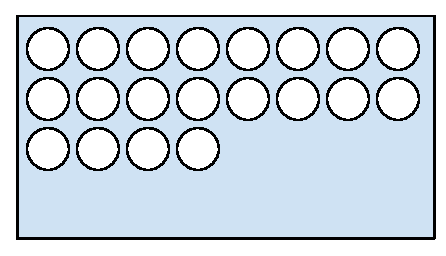
\includegraphics[width=0.5 \columnwidth,keepaspectratio]{figures/block.pdf}
    \caption{A block containing ordered transactions. We will draw a block using a rectangle
             and a transaction using a circle.}
    \label{fig.block}
\end{figure}

When a transaction makes it into a block, we term the transaction
\emph{confirmed}~\index{Confirmation}. An honest party invokes the \emph{read} functionality
of its ledger, only confirmed transactions are reported. This ensures that ledgers
are consistent, salvaging safety. Liveness is guaranteed from the fact that an honest
block will eventually appear, and this will cause all the transactions in the mempool to
become confirmed.

\section{Chain of Blocks}

Similar to transactions, we give blocks identifiers, which are the hashes of their contents.
A blockid of block $B$ is the value $H(B)$. Contrary to transactions, these blockids will
generally be a small value, because they all satisfy the proof-of-work equation. Therefore,
these hashes will begin with a run of $0$s.

At this point, we have introduced blocks that function as tickets to allow for the spaced-out
broadcasting of transactions. However, our system is not yet safe. There's a problem: While
the proof-of-work process ensures that the adversary gets a block in regular spaced out
intervals, the adversary is not guaranteed to use these block at the time of issuance.
Instead, the adversary could \emph{withhold} a couple of blocks and broadcast them all later
in close succession, and in particular closer than $\Delta$ apart in time. This defeats the
purpose we set to achieve. The attack stems from the ability of the adversary to use blocks
that are stale and have been set aside for long. We can resolve the issue by requiring
each block to be \emph{fresh}. We can do this by having the block include, in addition to
its transactions, a pointer to a previous recent block. This pointer, denoted by $s$,
is the blockid of the previous block known to the miner, and is known as the \emph{previd}\index{previd}.
Our modified block format is now $B = s \concat \overline{x} \concat \ctr$. Note that,
similarly to before, the adversary cannot retroactively change $s$ after mining a block,
because this will invalidate the proof-of-work. This helps with freshness: If a block $B$ is
old and includes a pointer $s$ to an even older block, this $s$ cannot be retroactively
chnaged to point to a newer block to make $B$ appear fresh. The final proof-of-work algorithm
illustrated in Algorithm~\ref{alg.mine-block}.
accepts both $s$ and $\overline{x}$ as parameters and tries to find a $\ctr$ that
satisfies the proof-of-work equation.

\import{./}{algorithms/alg.mine-block}

Because each block points to a previous block, the blocks form a chain. This is known
as the \emph{blockchain}\index{Blockchain} and is illustrated in Figure~\ref{fig.chain}.
The arrows follow the direction of the pointers, pointing from one block to the block
it refers to. While the pointers have a right-to-left direction, the blockchain was
produced from left-to-right. From now on, we will draw blocks as simple squares,
omitting the respective transactions inside for brevity.

\begin{figure}[h]
    \centering
    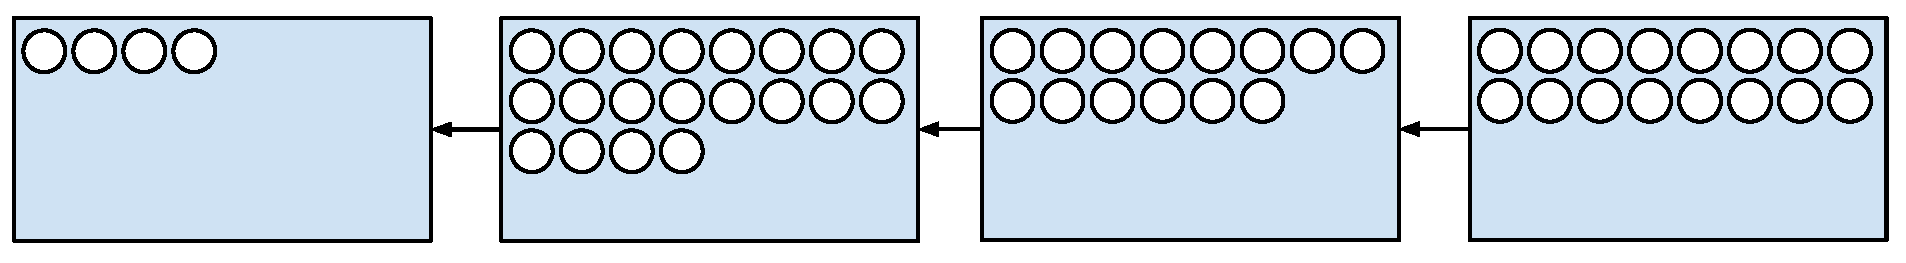
\includegraphics[width=1 \columnwidth,keepaspectratio]{figures/the-chain.pdf}
    \caption{A chain of blocks. The blocks were mined from left to right.}
    \label{fig.chain}
\end{figure}

Because the hash
of a block cannot be predicted prior to the proof-of-work actually taking place (otherwise
proof-of-work would be solvable by a faster algorithm than exhaustive search), the value
$s$ of the previd must be computed prior to the value $H(s \concat \overline{x} \concat \ctr)$.
In other words, the previd $s$ must already be known when mining for a new block that includes
$s$ as its previd. Blocks are mined in the order they appear. The pointers between blocks
in the chain are \emph{causality links}. They point backwards in time. The blockchain grows
forward in time and defines an \emph{arrow of time}. When we observe a blockchain, we can
deduce that all of its blocks were mined one after the other in the order that we observe
them.

% In particular, $Pr[H(B) \leq T] = \frac{T}{2^{\kappa}}$ for any arbitrary $B$.
% In the network, $T$ is fixed and hard-coded for honest parties. The value is chosen such that the time it takes for a node in the network to find a solution to the Proof-of-Work equation is around $\Delta$.

\section{Genesis}

We've added pointers between blocks to ensure freshness, and each block attests about
its freshness by a pointer to a recent block. But what about the freshness of the first
block on the chain? That first block cannot have a pointer to a parent block. How do we
ensure its freshness? In particular, how do we prevent an adversary from having produced
many blocks in secret prior to the blockchain protocol even being announced, anticipating
its announcement, perhaps in collusion with the creator of the protocol? To prove the
freshness of the first block, the first block contains a reference which ties the theoretical
and mathematical world of the blockchain with real world events. The first block, known as
the \emph{genesis block}\index{Genesis}, or simply \emph{genesis}, contains in its metadata
the headline of a recent newspaper describing impactful and unpredictable world events.
Because these data are committed into the proof-of-work of the genesis block, similarly
to the values $s$ and $\ctr$, they cannot be retroactively changed without invalidating
the proof-of-work. This is the way of the protocol creator indicating there's
\emph{nothing up his sleeve}, and that the genesis block was produced \emph{after}
a certain point in time. This is an \emph{anchor in time} and guards against the fear
of \emph{premining attacks}\index{Premining}, situations in which the protocol inventor
is adversarial and has mined blocks prior to making the protocol public. The genesis
block is denoted $\mathcal{G}$.
\glsxtrnewsymbol[description={genesis}]{genesis}{$\mathcal{G}$}\glsadd{genesis}

The Bitcoin genesis block was mined on January 3rd, 2009 and contains the following quote:

\begin{quote}
  The Times 03/Jan/2009 Chancellor on brink of second bailout for banks
\end{quote}

The quote is both an anchor in time and a political message by Satoshi Nakamoto. The
frontpage of The Times newspaper of that day appears in Figure~\ref{fig.thetimes}.

\begin{figure}[h]
    \centering
    
\includegraphics[width=1 \columnwidth,keepaspectratio]{figures/thetimes.jpg}
    \caption{The genesis block contains metadata with a time anchor to real-world events.}
    \label{fig.thetimes}
\end{figure}

\section{Mining}

Honest parties \emph{constantly} attempt to mine blocks by following the mining algorithm.
The steps that an honest miner follows are as follows:

\begin{enumerate}
  \item Maintain a consistent local mempool $\overline{x}$ of transactions.
  \item Attempt to mine a block $B = s \conc \overline{x} \conc \ctr$ by finding a $\ctr$ that satisfies $H(B) \leq T$.
  \item If mining is successful, broadcast the newly created block $B$.
  \item Otherwise, keep mining.
\end{enumerate}

The honest parties keep mining even if their mempool is empty. This means that the blockchain
might consist even of empty blocks.

\section{Problems}
TBD

\section{Further Reading}

Proof-of-Work was invented long before blockchains, in 1992, by Cynthia Dwork and Moni Naor
in their seminal paper \emph{Pricing via Processing or Combatting Junk Mail}~\cite{pow} published
in CRYPTO '92. Satoshi Nakamoto invented the blockchain by using proof-of-work as a building block.
